\newpage
\section{Resultados}

Nesta seção são apresentados os resultados obtidos para a trajetória, a cinemática inversa, as velocidades, os torques e os controladores. Os valores foram retirados de uma execução completa da simulação, considerando o aplicador de $3{,}0\,\text{kg}$ e o TCP localizado a $0{,}15\,\text{m}$ do flange.

\subsection{Trajetória executada}

A sequência realizada foi: estação de ferramentas $\rightarrow$ retângulo $\rightarrow$ estação $\rightarrow$ losango $\rightarrow$ estação $\rightarrow$ círculo $\rightarrow$ estação $\rightarrow$ arco $\rightarrow$ estação. As cores do rastro permitem identificar os trechos de pintura e os movimentos de transição.

\begin{figure}[H]
    \centering
    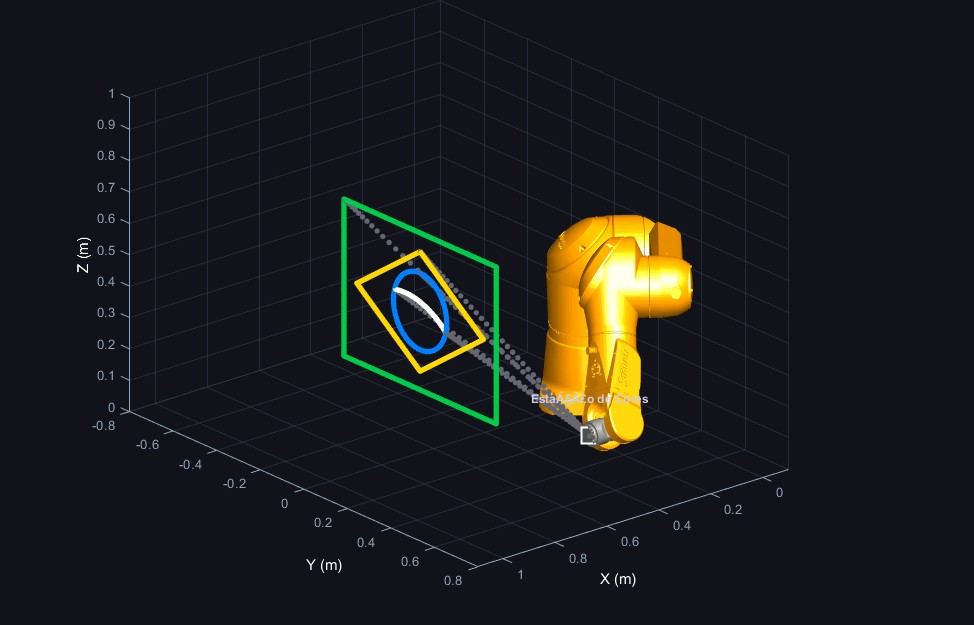
\includegraphics[width=0.72\linewidth]{Imagens/simulacao.jpeg}
    \caption{Execução da trajetória pelo Stäubli TX90.}
    \label{fig:simulacao_final}
\end{figure}

A trajetória completa possui 1696 pontos, com intervalo de amostragem de $0{,}04\,\text{s}$. Como a primeira amostra ocorre em $t=0$, a duração total é

\begin{equation}
T_{\mathrm{ciclo}}=(N-1)\Delta t=(1696-1)\,0{,}04=67{,}80\,\text{s}.
\end{equation}

A maior velocidade cartesiana foi de $0{,}3474\,\text{m/s}$ e a maior aceleração foi de $0{,}5986\,\text{m/s}^2$. Esses valores permaneceram abaixo dos limites de $0{,}35\,\text{m/s}$ e $0{,}60\,\text{m/s}^2$ usados nas transições. Durante a pintura foram aplicados limites menores, de $0{,}12\,\text{m/s}$ e $0{,}30\,\text{m/s}^2$.

\begin{figure}[H]
    \centering
    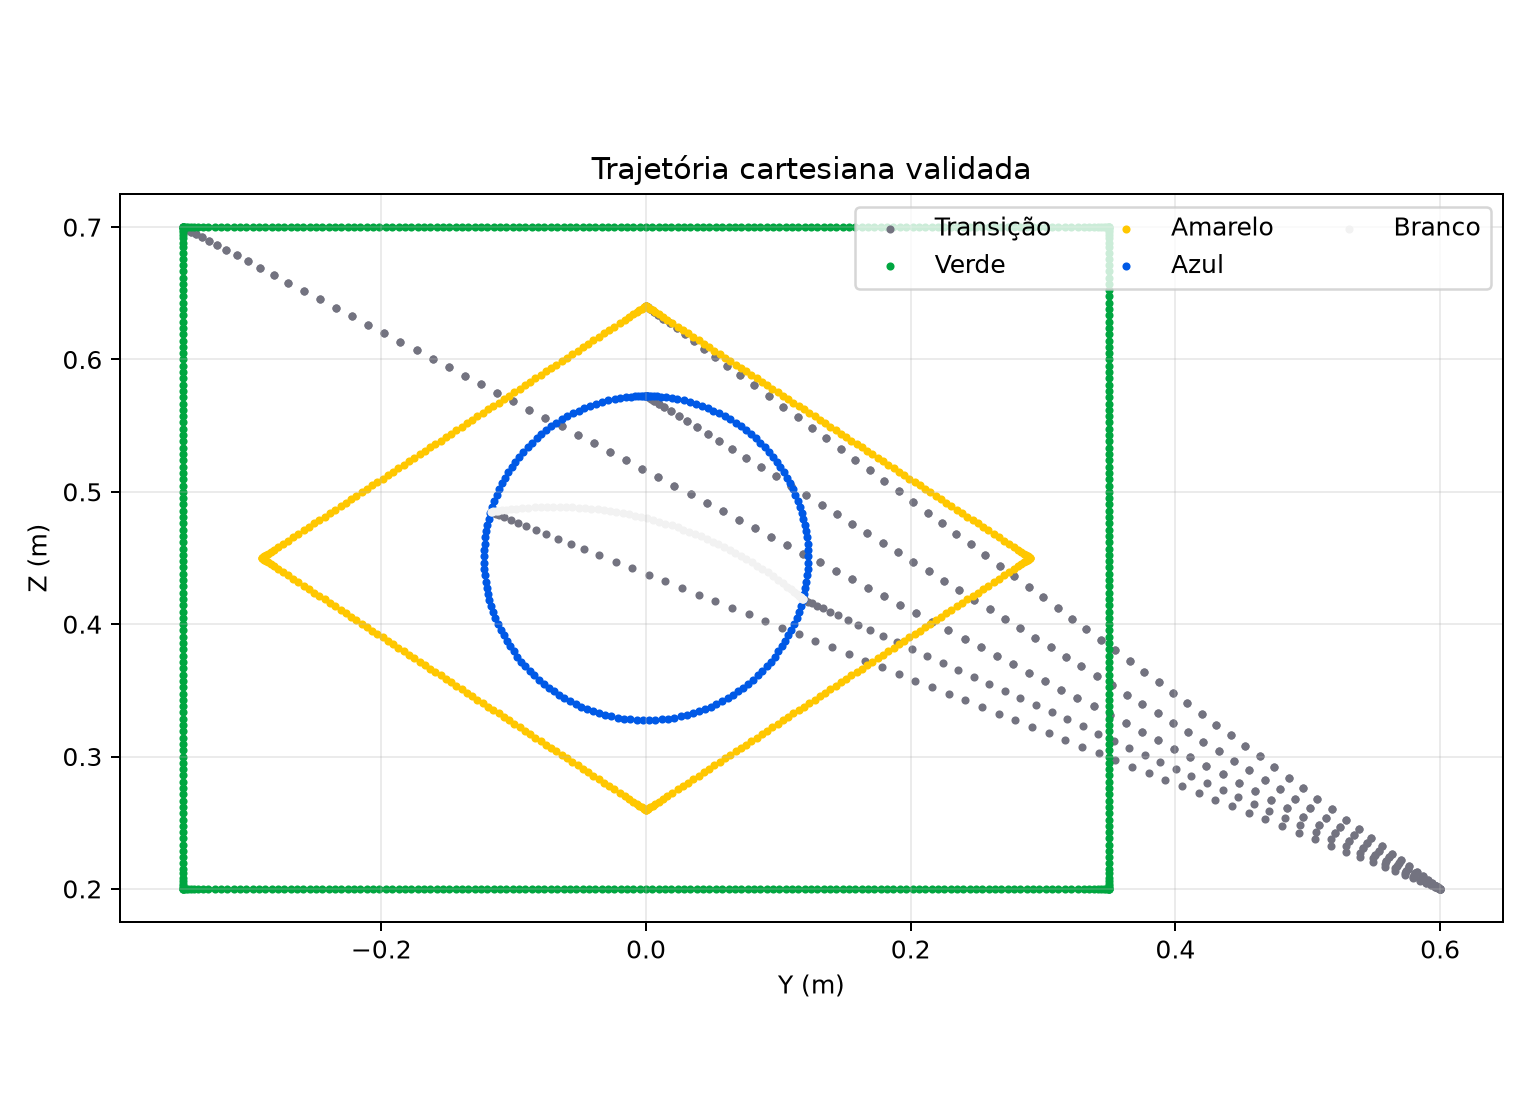
\includegraphics[width=0.78\linewidth]{Imagens/trajetoria_validada.png}
    \caption{Trajetória cartesiana completa, incluindo os contornos e as transições.}
    \label{fig:trajetoria_validada}
\end{figure}

\subsection{Alcance e cinemática inversa}

A nuvem de pontos da Figura~\ref{fig:workspace_validado} foi obtida a partir de configurações dentro dos limites articulares. Ela serve como uma representação aproximada do espaço de trabalho, enquanto a alcançabilidade da tarefa foi verificada individualmente pela cinemática inversa e pela reconstrução de cada pose com a cinemática direta.

\begin{figure}[H]
    \centering
    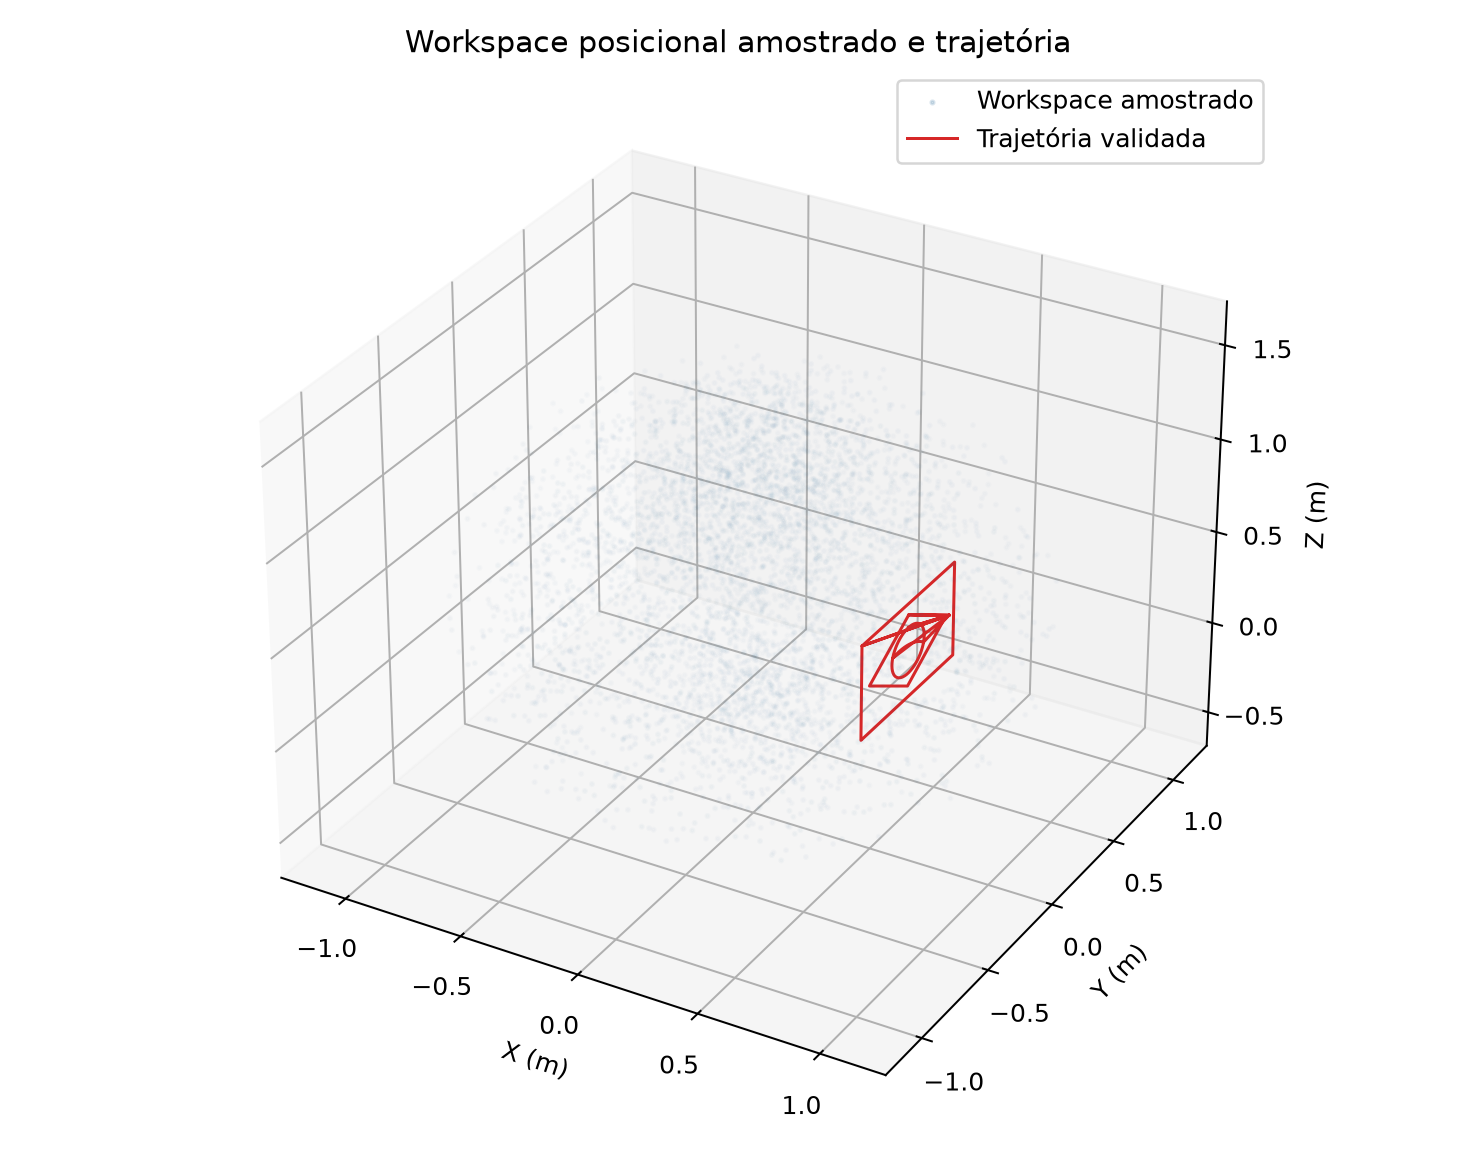
\includegraphics[width=0.78\linewidth]{Imagens/workspace_validado.png}
    \caption{Espaço de trabalho amostrado e trajetória verificada ponto a ponto.}
    \label{fig:workspace_validado}
\end{figure}

As 1696 poses apresentaram solução. O erro máximo de posição ficou abaixo de $0{,}001\,\text{mm}$, enquanto o maior erro de orientação foi de $1{,}414\times10^{-7}\,\text{rad}$. Também foi calculado o menor valor singular do Jacobiano ao longo da trajetória, obtendo-se

\begin{equation}
\min_t\sigma_{\min}\bigl(J(q(t))\bigr)=0{,}1143.
\end{equation}

Como esse valor permaneceu diferente de zero, não foi observada perda de posto do Jacobiano nas poses avaliadas.

\subsection{Velocidades e torques}

Os maiores módulos de velocidade articular foram $0{,}910$, $0{,}683$, $0{,}911$, $1{,}038$, $0{,}693$ e $0{,}840\,\text{rad/s}$ para J1 a J6, respectivamente. Todos permaneceram abaixo dos limites definidos no modelo do robô.

Os torques foram calculados pela dinâmica inversa a partir de $q(t)$, $\dot q(t)$ e $\ddot q(t)$. A Tabela~\ref{tab:torques_dinamica_inversa} apresenta os valores máximos e RMS obtidos durante o ciclo.

\begin{table}[H]
\centering
\small
\caption{Torques obtidos por dinâmica inversa.}
\label{tab:torques_dinamica_inversa}
\begin{tabular}{ccccc}
\toprule
Junta & Máximo (Nm) & RMS (Nm) & Limite (Nm) & Utilização máxima \\
\midrule
J1 & 5,08   & 1,40  & 318 & 1,6\% \\
J2 & 105,50 & 68,34 & 166 & 63,5\% \\
J3 & 31,82  & 19,19 & 76  & 41,9\% \\
J4 & 5,09   & 1,97  & 34  & 15,0\% \\
J5 & 6,58   & 6,11  & 29  & 22,7\% \\
J6 & 0,016  & 0,015 & 11  & 0,15\% \\
\bottomrule
\end{tabular}
\end{table}

O maior esforço ocorreu em J2, com $105{,}50\,\text{Nm}$, correspondendo a $63{,}5\%$ do limite dessa junta. Esse resultado é coerente com a posição de J2 na cadeia, pois ela sustenta uma parte importante do braço e da ferramenta contra a gravidade. Nenhuma junta ultrapassou o limite de esforço adotado.

\begin{figure}[H]
    \centering
    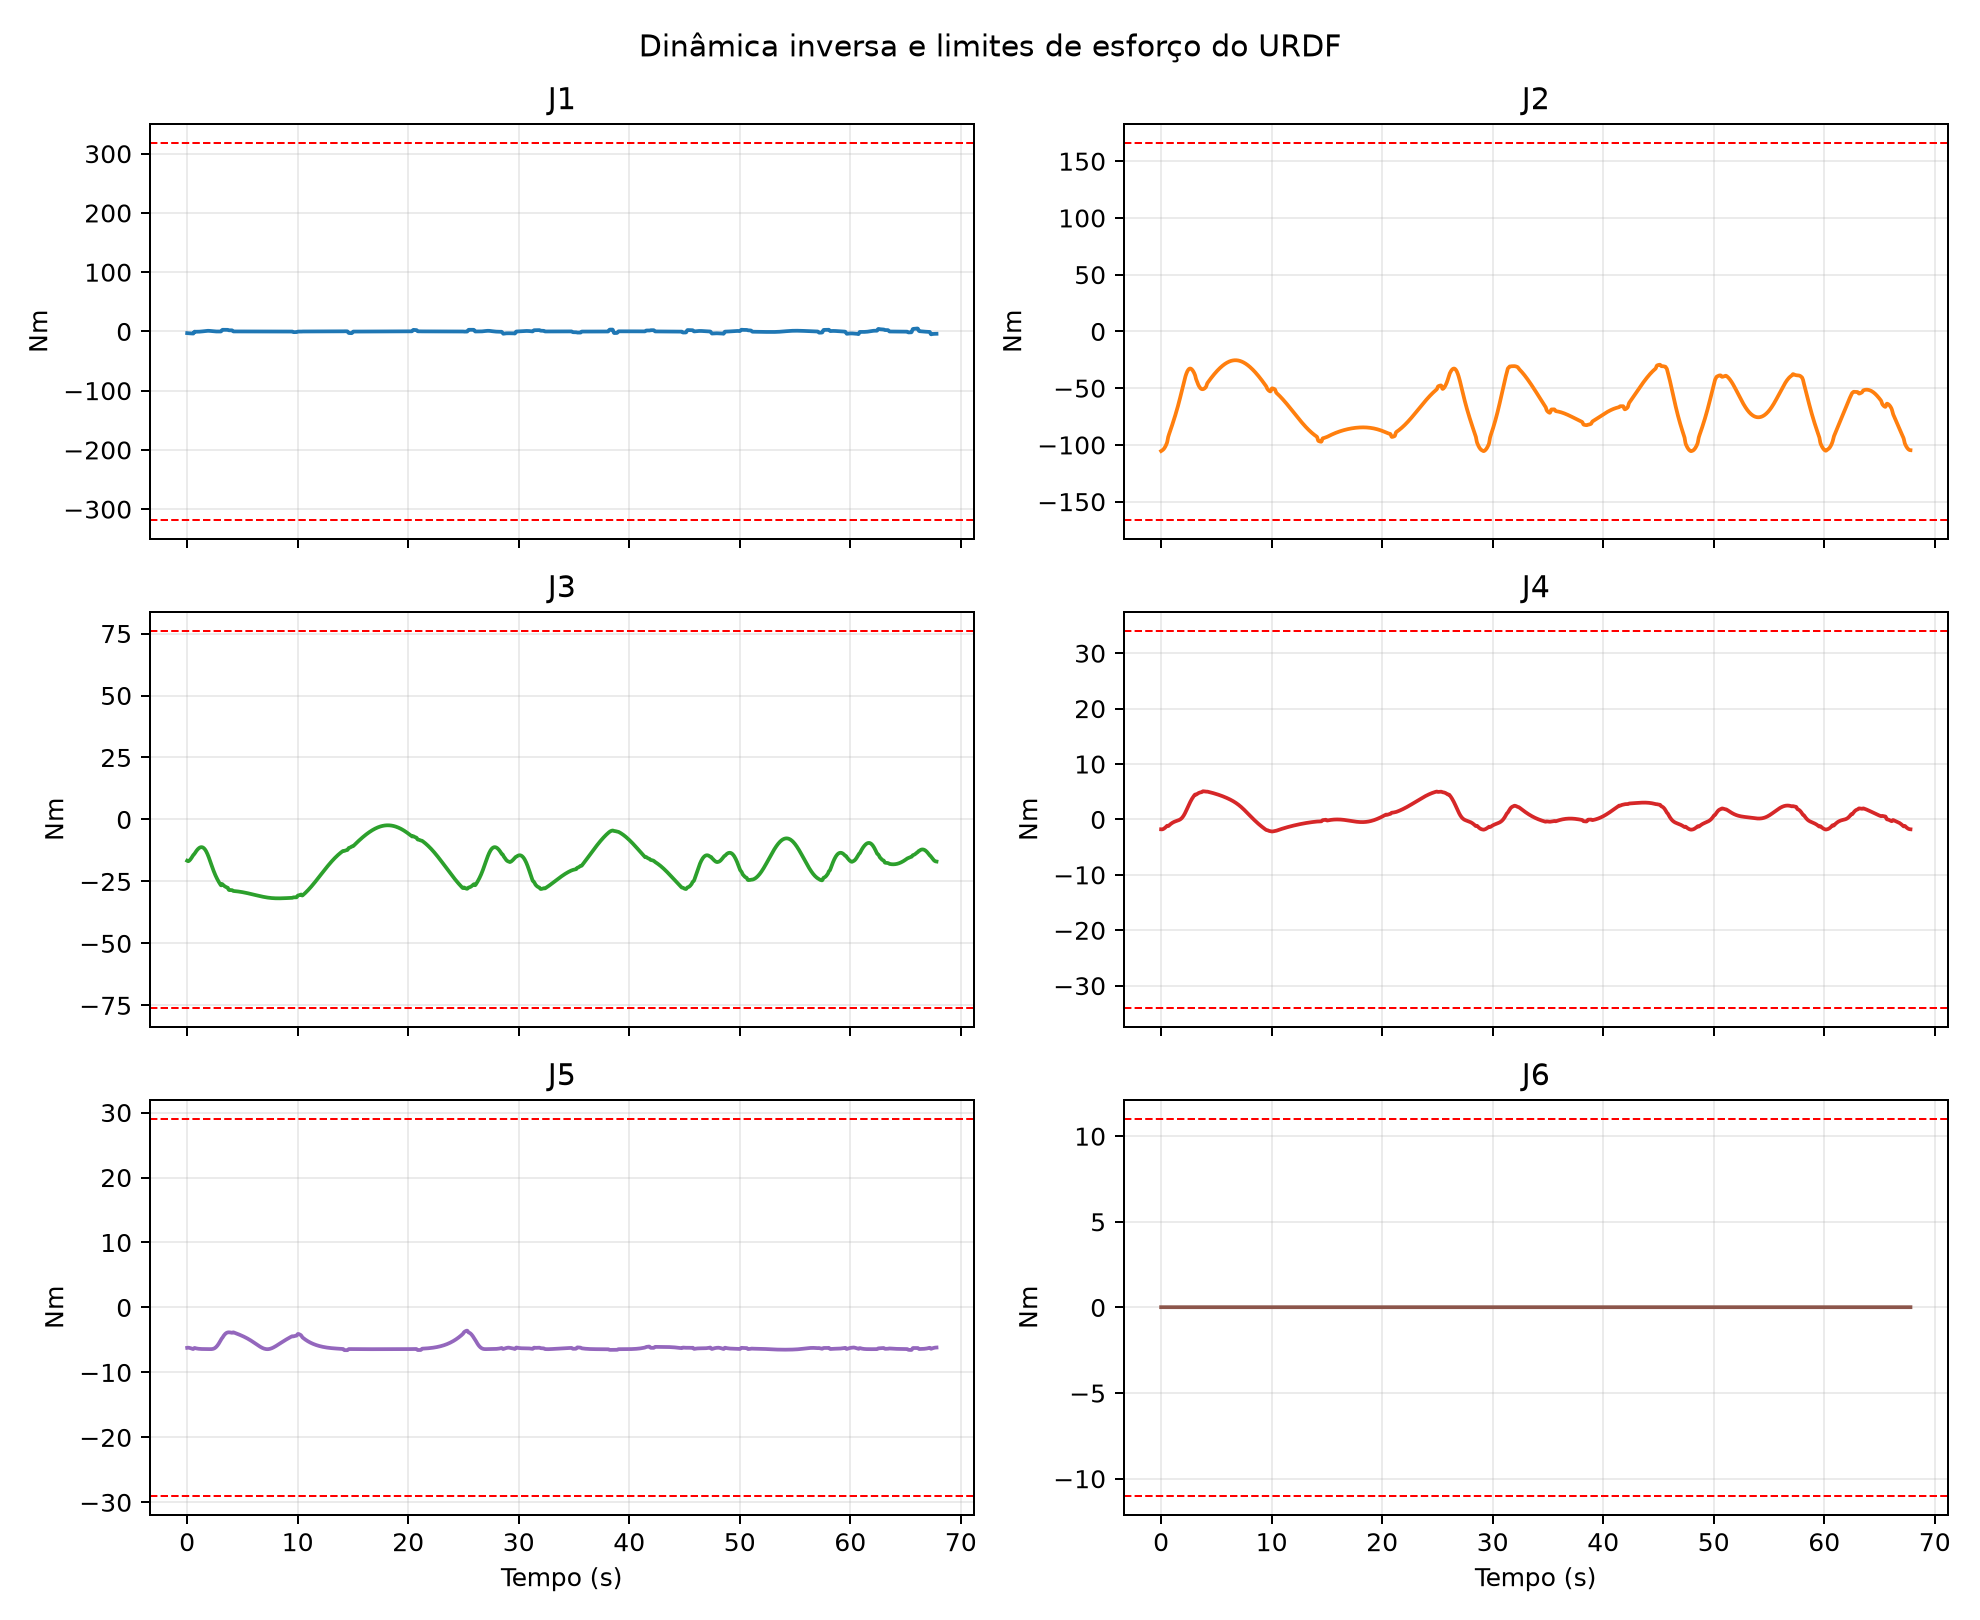
\includegraphics[width=0.90\linewidth]{Imagens/torques_limites.png}
    \caption{Torques calculados e limites de esforço considerados para cada junta.}
    \label{fig:torques_limites}
\end{figure}

\subsection{Controle da trajetória}

Foram avaliadas duas formas de controle: PD com compensação de gravidade e controle por torque computado. A comparação foi feita pelo erro RMS de posição de cada junta, apresentado na Tabela~\ref{tab:controle_comparacao}.

\begin{table}[H]
\centering
\small
\caption{Erro RMS de rastreamento dos controladores.}
\label{tab:controle_comparacao}
\begin{tabular}{ccc}
\toprule
Junta & PD + gravidade (rad) & Torque computado (rad) \\
\midrule
J1 & 0,006886 & 0,003301 \\
J2 & 0,006256 & 0,002702 \\
J3 & 0,009007 & 0,002436 \\
J4 & 0,027990 & 0,003738 \\
J5 & 0,028400 & 0,001746 \\
J6 & 0,005400 & 0,002060 \\
\bottomrule
\end{tabular}
\end{table}

Os dois controladores acompanharam a referência, mas o torque computado apresentou erro RMS menor em todas as juntas. A diferença foi mais evidente em J4 e J5, mostrando a vantagem de considerar, além da gravidade, os termos de inércia e Coriolis do manipulador.

\begin{figure}[H]
    \centering
    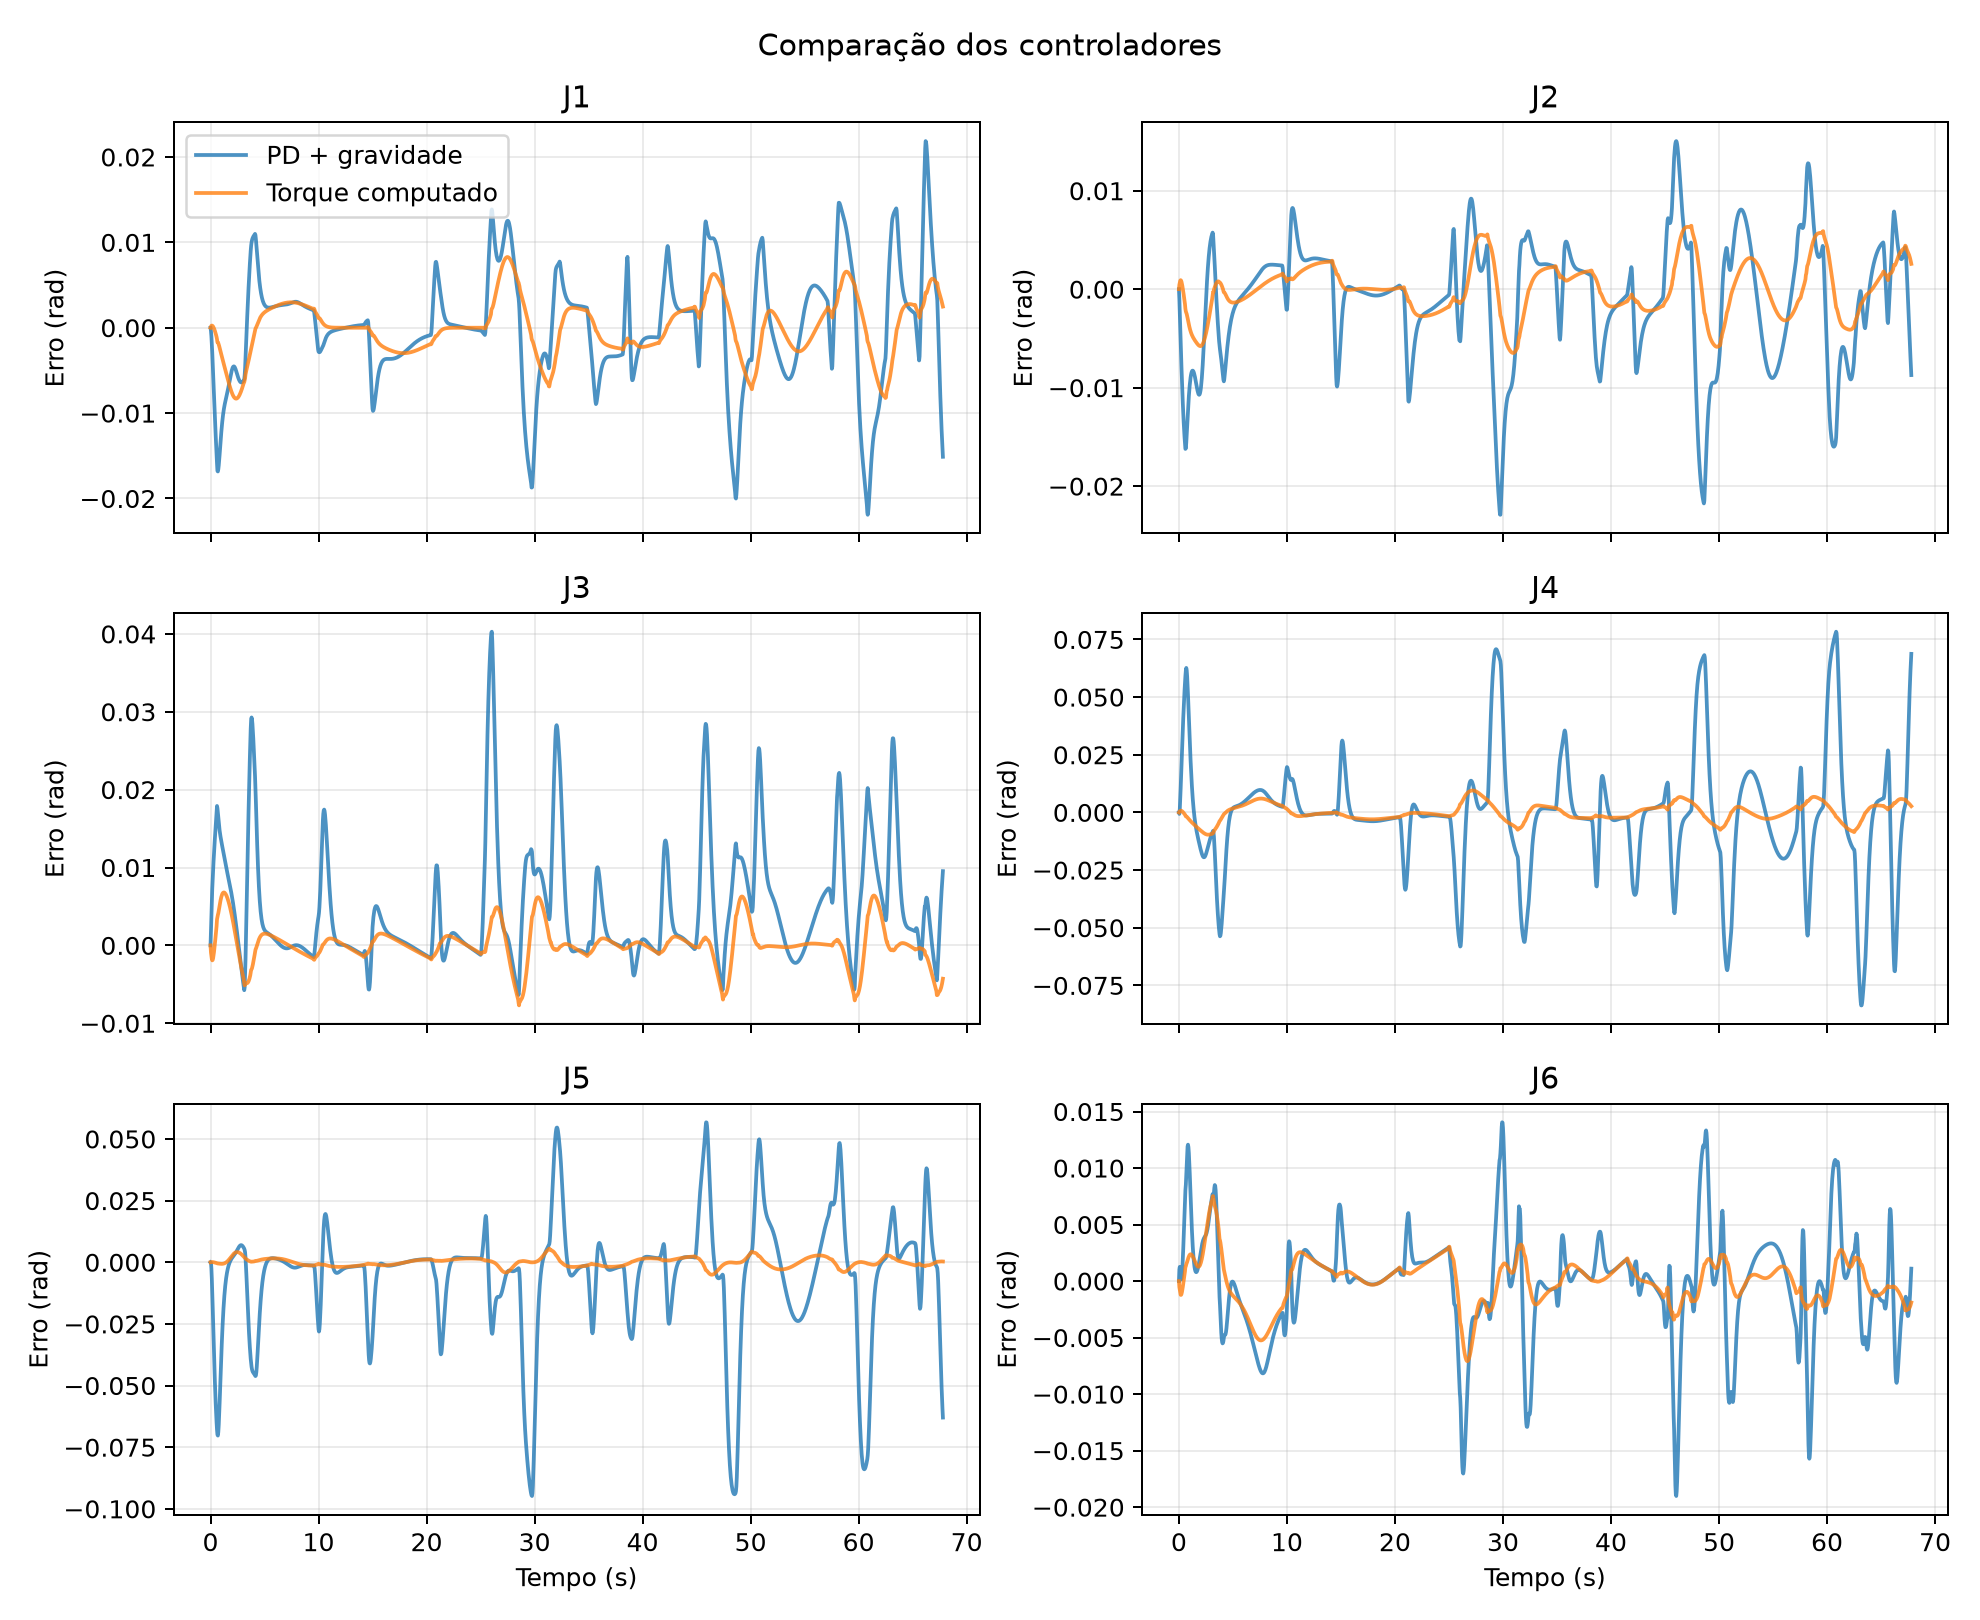
\includegraphics[width=0.92\linewidth]{Imagens/comparacao_controle.png}
    \caption{Comparação dos erros de rastreamento dos dois controladores.}
    \label{fig:comparacao_controle}
\end{figure}

\subsection{Implementação computacional}

A simulação foi desenvolvida no MATLAB com a Robotics System Toolbox. O modelo do TX90 foi importado em formato URDF e recebeu a massa, o centro de massa e o comprimento do aplicador. A trajetória foi formada pelos pontos do retângulo, losango, círculo e arco, ligados à estação de ferramentas por movimentos com perfil LSPB. Em seguida, foram resolvidas a cinemática inversa, a dinâmica inversa e as duas leis de controle.

Para facilitar o entendimento, o funcionamento geral pode ser separado nos blocos descritos a seguir.

\paragraph{Carregamento do robô e da ferramenta}
O primeiro bloco importa o modelo URDF do TX90, define a gravidade e obtém os limites das seis juntas. Em seguida, é acrescentado o aplicador de $3{,}0\,\text{kg}$, com seu centro de massa e o TCP localizado a $0{,}15\,\text{m}$ do flange. Dessa forma, a cinemática e a dinâmica passam a considerar a ferramenta utilizada na tarefa.

\paragraph{Definição da bandeira e da estação}
O segundo bloco define os pontos do retângulo, losango, círculo e arco, além da posição da estação de ferramentas. Cada forma é representada por pontos cartesianos no plano da bandeira, e os deslocamentos entre as formas passam obrigatoriamente pela estação.

\paragraph{Geração da trajetória}
Para cada trecho é calculado um perfil LSPB a partir do comprimento, da velocidade máxima, da aceleração máxima e do intervalo de amostragem. Os trechos de pintura utilizam limites menores que os movimentos de transição. Ao final, todas as posições, velocidades e acelerações são reunidas em uma única trajetória temporal.

\paragraph{Cinemática inversa e validação}
A cinemática inversa é resolvida para cada pose desejada do TCP, sempre utilizando a solução anterior como estimativa inicial. Essa escolha ajuda a manter a continuidade do movimento. Depois, a cinemática direta é aplicada às soluções encontradas para calcular os erros de posição e orientação e verificar se a trajetória foi realmente reproduzida.

\paragraph{Velocidades, acelerações e dinâmica}
As velocidades e acelerações articulares são obtidas por diferenças finitas. Com $q(t)$, $\dot q(t)$ e $\ddot q(t)$, são calculados os torques necessários pela dinâmica inversa. Os valores máximos são então comparados com os limites de esforço de cada junta.

\paragraph{Controle e apresentação dos resultados}
Por fim, a trajetória é simulada com o controlador PD com compensação de gravidade e com o controlador por torque computado. Os erros de rastreamento são calculados para as seis juntas, enquanto a animação apresenta o movimento do robô e o rastro correspondente a cada cor da bandeira.

\newpage
\section{Discussão}

Os resultados mostram que o TX90 consegue executar a trajetória proposta dentro das condições adotadas. Todos os pontos tiveram solução de cinemática inversa, não houve indicação de singularidade nas poses avaliadas e os limites de velocidade e torque foram respeitados. O perfil LSPB também permitiu manter trechos de velocidade aproximadamente constante com aceleração e desaceleração suaves.

O torque de J2 foi o mais próximo de seu limite, mas ainda apresentou uma margem de $36{,}5\%$. Essa margem é suficiente para o cenário simulado, porém não deve ser interpretada como capacidade disponível para qualquer ferramenta ou trajetória. O torque depende da massa, do centro de massa, da aceleração e da configuração do braço, sendo necessária uma nova análise caso algum desses parâmetros seja alterado.

O controle por torque computado apresentou o melhor rastreamento, pois utiliza um modelo mais completo da dinâmica. Mesmo assim, o PD com compensação de gravidade também apresentou erros pequenos e pode ser uma alternativa mais simples quando não se dispõe de um modelo dinâmico suficientemente preciso.

\subsection{Dificuldades encontradas}

 Alguns pontos que podem ser discutidos são a obtenção do modelo do robô, a definição dos referenciais, a solução da cinemática inversa, a geração da trajetória, o cálculo dos torques e a sintonia dos controladores.

\subsection{Limitações e próximos passos}

A validação realizada é numérica e considera o robô como um sistema de corpos rígidos. Não foram incluídos efeitos como colisões, flexibilidade, dinâmica das mangueiras, atraso dos atuadores ou variações nos parâmetros de massa. A ferramenta de $3{,}0\,\text{kg}$ também foi adotada como uma estimativa de projeto.

Para aproximar o estudo de uma aplicação real, os próximos passos seriam medir a massa, o centro de massa e a inércia do aplicador; calibrar os referenciais da base, da bandeira e do TCP; inserir a geometria da célula para verificar colisões; e realizar testes em baixa velocidade antes da execução completa.

A simulação atual representa o contorno das partes da bandeira. Para realizar o preenchimento, seria necessário gerar passadas paralelas no interior de cada região, considerando a largura do jato, a distância até a peça e a sobreposição entre passadas. Essa alteração aumentaria o número de segmentos e o tempo de ciclo, mas poderia ser feita sem modificar o modelo cinemático e dinâmico já desenvolvido.

Após o período de maior demanda relacionado à Copa, a mesma linha poderia ser reconfigurada para pintar outros padrões ou para atividades como acabamento, inspeção e movimentação de componentes. Os limites de torque do modelo chegam a $318\,\text{Nm}$ na junta de maior capacidade, o que permite considerar tarefas mais exigentes do que o traçado da bandeira. Entretanto, cada nova aplicação precisaria de uma verificação própria, principalmente para J2, que foi a junta mais solicitada neste trabalho.

\subsection{Contribuições da equipe}

\begin{table}[H]
\centering
\small
\caption{Contribuições dos integrantes.}
\begin{tabularx}{\textwidth}{|p{5.0cm}|X|}
\hline
\textbf{Integrante} & \textbf{Contribuição} \\ \hline
Gabriel Erick Matheus Imamura & Revisão bibliográfica, contextualização da aplicação, pesquisa e comparação de manipuladores e organização das fontes. \\ \hline
Matheus Gasques Siqueira & A confirmar pela equipe antes da entrega. \\ \hline
Gabriel Zanette Cipriano & A confirmar pela equipe antes da entrega. \\ \hline
Lucca Ewertom Ryuichi Hirakawa & A confirmar pela equipe antes da entrega. \\ \hline
João Victor Pomiglio de Oliveira & A confirmar pela equipe antes da entrega. \\ \hline
\end{tabularx}
\end{table}

\subsection{Código MATLAB utilizado}

O código completo utilizado para gerar a trajetória, calcular a cinemática inversa, avaliar a dinâmica e simular os controladores é apresentado a seguir. Ele foi organizado em múltiplos arquivos, com uma função pública por arquivo, conforme a convenção do MATLAB: o script principal define todos os parâmetros do projeto e orquestra as etapas, e cada etapa é implementada em uma função própria.

\begingroup
\singlespacing
\lstinputlisting[caption={Script principal da simulação (simulacaoTX90.m).},label={lst:simulacaoTX90}]{\dirSimulacao/simulacaoTX90.m}
\lstinputlisting[caption={Carregamento do robô e da ferramenta (+robotica/carregarRobo.m).},label={lst:carregarRobo}]{\dirSimulacao/funcoes/+robotica/carregarRobo.m}
\lstinputlisting[caption={Geração da trajetória cartesiana com perfil LSPB (+trajetoria/gerarTrajetoria.m).},label={lst:gerarTrajetoria}]{\dirSimulacao/funcoes/+trajetoria/gerarTrajetoria.m}
\lstinputlisting[caption={Cinemática inversa com validação por cinemática direta (+robotica/resolverCinematicaInversa.m).},label={lst:resolverCinematicaInversa}]{\dirSimulacao/funcoes/+robotica/resolverCinematicaInversa.m}
\lstinputlisting[caption={Dinâmica inversa e análise dos torques (+robotica/calcularTorques.m).},label={lst:calcularTorques}]{\dirSimulacao/funcoes/+robotica/calcularTorques.m}
\lstinputlisting[caption={Controladores em malha fechada (+controle/simularControlador.m).},label={lst:simularControlador}]{\dirSimulacao/funcoes/+controle/simularControlador.m}
\lstinputlisting[caption={Métricas de rastreamento do controlador (+controle/analisarControle.m).},label={lst:analisarControle}]{\dirSimulacao/funcoes/+controle/analisarControle.m}
\lstinputlisting[caption={Verificação da área de trabalho (+areaTrabalho/verificarAreaTrabalho.m).},label={lst:verificarAreaTrabalho}]{\dirSimulacao/funcoes/+areaTrabalho/verificarAreaTrabalho.m}
\lstinputlisting[caption={Gráficos de resultados (+visualizacao/plotarResultados.m).},label={lst:plotarResultados}]{\dirSimulacao/funcoes/+visualizacao/plotarResultados.m}
\lstinputlisting[caption={Animação 3D da execução (+visualizacao/animarRobo.m).},label={lst:animarRobo}]{\dirSimulacao/funcoes/+visualizacao/animarRobo.m}
\lstinputlisting[caption={Helper de estilo: figura com tema escuro (+visualizacao/criarFiguraEscura.m).},label={lst:criarFiguraEscura}]{\dirSimulacao/funcoes/+visualizacao/criarFiguraEscura.m}
\lstinputlisting[caption={Helper de estilo: eixo com tema escuro (+visualizacao/estilizarEixoEscuro.m).},label={lst:estilizarEixoEscuro}]{\dirSimulacao/funcoes/+visualizacao/estilizarEixoEscuro.m}
\endgroup
